\section{On-policy Control with Approximation}
\subsection{Episodic Semi-gradient Control}
In the previous chapter, we used \textit{semi-gradient methods}, namely semi-gradient TD(0), to approximate the state value function $\hat{v}_\pi$. Now, for the control setting, we want to instead approximate the state-action value function $\hat{q}_\pi$ so we can take greedy actions w.r.t it. The general gradient descent update for the action-value prediction is
\begin{equation}
\textbf{w}_{t+1} \doteq \textbf{w}_t + \alpha\left[U_t - \hat{q}(S_t, A_t, \textbf{w}_t)\right] \nabla \hat{q}(S_t, A_t, \textbf{w}_t)
\end{equation}

We can then use our function approximation to select actions greedily i.e. $A_{t+1}^* = \argmax_a \hat{q}(S_t, a, \textbf{w}_t)$. In the on-policy case (this chapter) this policy used for this selection must be the same as the one used for estimation (i.e. to obtain $U_t$). The algorithm for episode semi-gradient sarsa is shown in Figure \ref .

\begin{figure}[h!]
	\centering
	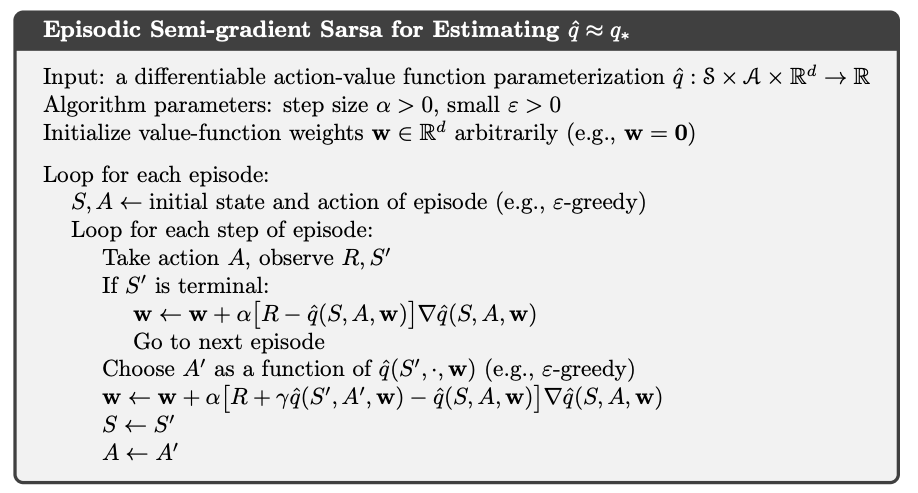
\includegraphics[width=\textwidth]{/chapter10_1}
	\caption{Episodic semi-gradient sarsa for estimating $\hat{q} \approx q_*$}
	\label{fig: 10_1}
\end{figure}

\subsection{Semi-gradient $n$-step Sarsa}
The $n$-step semi-gradient sarsa algorithm follows logically from the previous section. The $n$-step return becomes
\begin{equation}
G_{t:t+n} \doteq R_{t+1} + \gamma R_{t+2} + \cdots + \gamma^{n-1} + R_{t+n} + \gamma \hat{q}(S_{t+n}, A_{t+n}, \textbf{w}_{t+n-1})
\end{equation}

The $n$-step update becomes
\begin{equation}
\textbf{w}_{t+n} \doteq \textbf{w}_{t+n-1} + \alpha \left[G_{t:t+n} - \hat{q} (S_t, A_t, \textbf{w}_{t+n-1})\right] \nabla \hat{q}(S_t, A_t, \textbf{w}_{t+n-1})
\end{equation}

The algorithm is provided in Figure \ref{fig: 10_2}. Generally, an intermediate level of bootstrapping shows optimal performance.

\begin{figure}[h!]
	\centering
	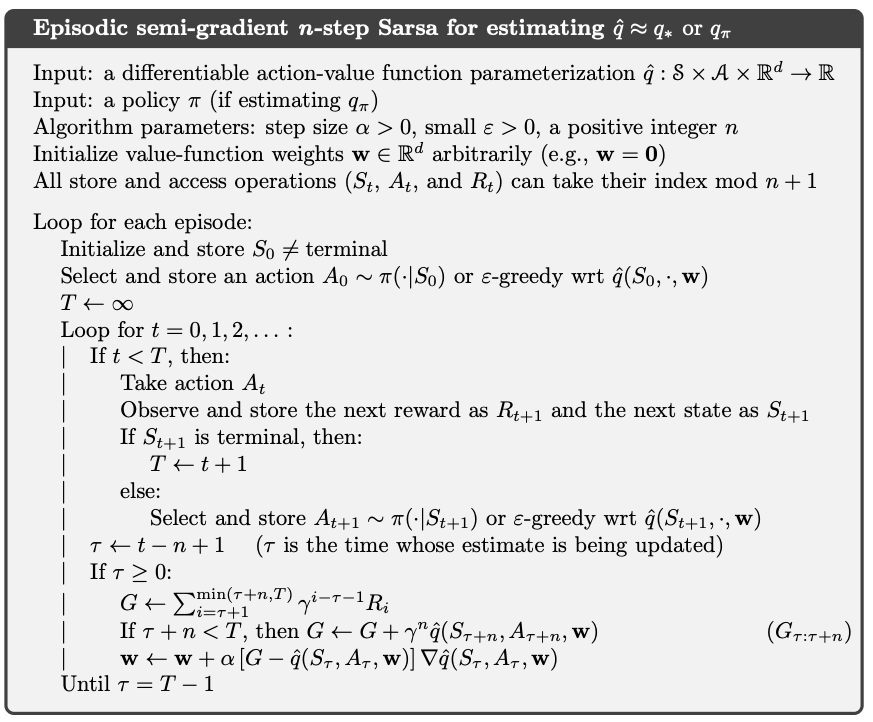
\includegraphics[width=0.8\textwidth]{/chapter10_2}
	\caption{Episodic semi-gradient $n$-step sarsa for estimating $\hat{q} \approx q_*$}
	\label{fig: 10_2}
\end{figure}

\subsection{Average Reward: A New Problem Setting for Continuing Tasks}
Until now we have considered two types of rewards: episodic and discounted (for continuing tasks). The average reward is a third task with no discounting, such that future rewards are valued just the same as present rewards. In the average-reward setting, the quality of a policy $\pi$ is defined as the average rate of reward, or simply \textit{average reward}, while following that policy, which we denote as $r(\pi)$
\begin{align}
r(\pi) &\doteq \lim_{h \rightarrow \infty}\frac{1}{h} \sum_{t=1}^{h} \mathbb{E} \left[R_t | S_0, A_{0:t-1} ~ \pi \right] \\
&= \lim_{t \rightarrow \infty} \mathbb{E} \left[R_t | S_0, A_{0:t-1} ~ \pi \right] \\
&= \sum_{s} \mu_\pi(s) \sum_{a} \pi(a|s) \sum_{s', r} p(s', r|s,a)r
\end{align}

The last equation holds if $\mu_\pi(s)$ exists and is independent of $S_0$, in other words if the MDP is \textit{ergodic} i.e. the long run expectation of being in a state depends only on the policy and the MDP transition probabilities.

We can order policies based on their average reward per timestep–$r(\pi)$– and all policies that attain the maximal reward rate are considered optimal.

In the average-reward setting, returns are defined in terms of differences between rewards and the average reward
\begin{equation}
G_t \doteq R_{t+1} - r(\pi) + R{t+2} - r(\pi) + R{t+3} - r(\pi) + \cdots
\end{equation}
known as the \textit{differential return} with corresponding value functions known as \textit{differential value functions}. This can be used to create new TD errors, the action-value error being
\begin{equation}
\delta_t \doteq R_{t+1} - \bar{R}_t + \hat{q}(S_{t+1}, A_{t+1}, \textbf{w}_t) - \hat{q}(S_t, A_t, \textbf{w}_t)
\end{equation}

where $\bar{R}_t$ is an estimate at time $t$ of the average reward $r(\pi)$. This error can be used to create a differential semi-gradient sarsa algorithm as shown in Figure \ref{fig: 10_3}
\begin{figure}[h!]
	\centering
	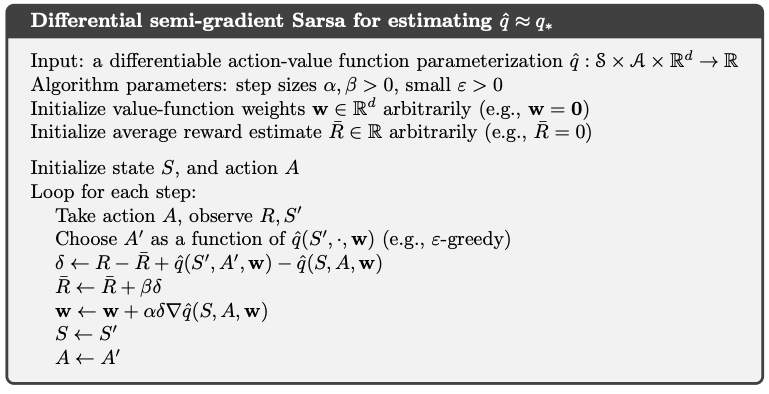
\includegraphics[width=\textwidth]{/chapter10_3}
	\caption{Differential semi-gradient sarsa for estimating $\hat{q} \approx q_*$}
	\label{fig: 10_3}
\end{figure}

\subsection{Deprecating the Discounted Setting}
Should we use the discounted reward or the average reward in continuous settings? It turns out there is no benefit to using discounting in the continuous setting, as, given a large enough sequences of rewards (infinite in the limit) we end up multiplying every reward by the same sequence of discounts $1 + \gamma + \gamma^2 + \gamma^3 + \gamma^4 + \cdots = \frac{1}{1 - \gamma}$.

The root cause of difficulties with the discounted control setting is that with function approximation we lose the policy improvement theorem from chapter 4. We can no longer say that if we change the policy to improve the discounted value of one state we are guaranteed to have improved the overall policy - errors in our function approximation mean we could have a detrimental effect on our value function elsewhere.

\subsection{Differential Semi-gradient $n$-step Sarsa}
For the $n$-step generalisation of Sarsa, we just need an expression for the $n$-step differential return with function approximation:
\begin{equation}
G_{t:t+n} \doteq R_{t+1} - \bar{R}_{t+n-1} + \cdots + R_{t+n} - \bar{R}_{t+n-1} - \hat{q}(S_{t+n}, A_{t+n}, \textbf{w}_{t+n-1}) 
\end{equation}

The pseudocode is given in Figure \ref{fig: 10_4}.

\begin{figure}[h!]
	\centering
	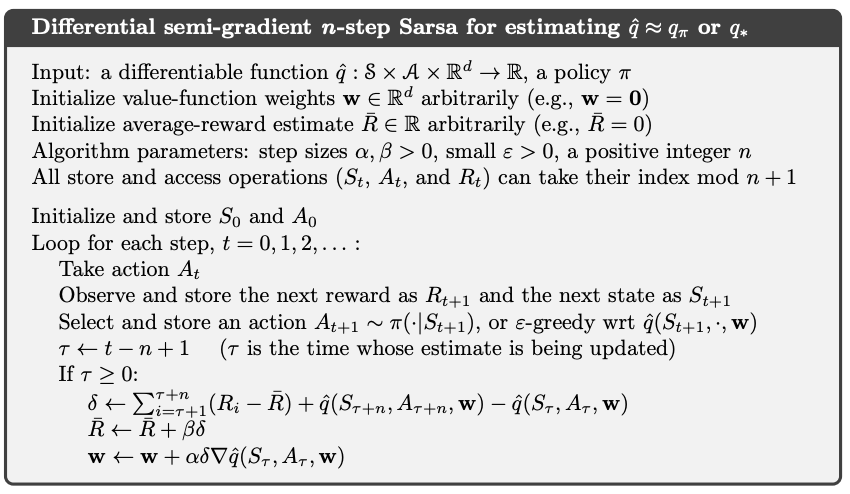
\includegraphics[width=\textwidth]{/chapter10_4}
	\caption{Differential semi-gradient $n$-step sarsa for estimating $\hat{q} \approx q_*$}
	\label{fig: 10_4}
\end{figure}

\subsection{Key Takeaways}
\begin{itemize}
\item In the episodic case, control with function approximation works the same as before, we find the approximate value function and act greedily.
\item In the continuing task setting we need to introduce a new reward–the average reward $r(\pi)$–which represents our expectation over the reward space.
\item Our updates are now governed by the \textit{differential reward} which is the difference between our observed reward and current best estimate for the average reward.
\item Discounting does not matter/work in the presence of approximations, as in this case, most policies cannot be represented by a value function. Instead, policies need to be ranked and the average reward $r(\pi)$ provides an effective way to do this.
\end{itemize}




